\documentclass[11pt]{extarticle}

% Packages
\usepackage{amsmath}
\usepackage[utf8]{inputenc}
\usepackage[russian]{babel}
\usepackage{geometry}
\usepackage{graphicx}

% Options
\graphicspath{ {../figures/} }
\geometry{left=2.5cm,right=2.5cm,top=2.5cm,bottom=2.5cm}
\setlength\parindent{0pt}

% Title
\title{
	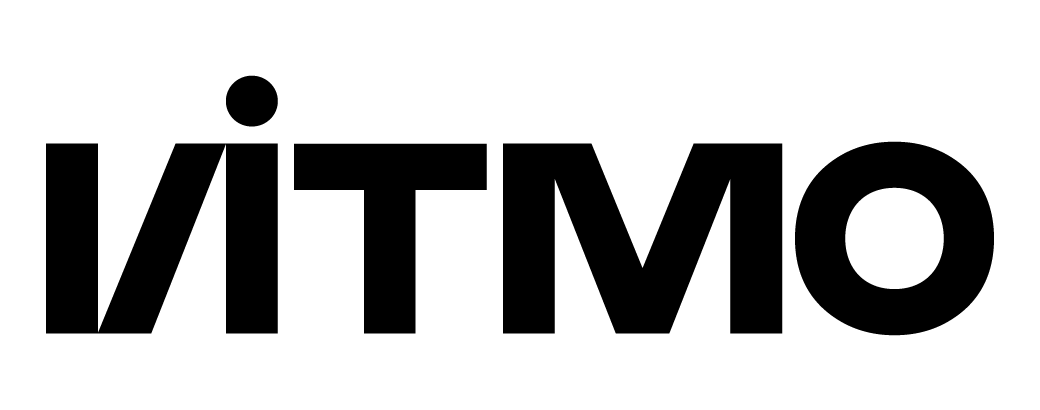
\includegraphics[scale=0.07]{logo}\\
	\vspace{0.5em}
	Языки программирования. Семантика и система типов\\
	\vspace{0.2em}
	\Large Теоретическое задание. Тема 1
}
\author{Бронников Егор}
\date{}


\begin{document}


% Титул


\maketitle

\vspace{-0.5cm}
\hrule
\vspace{0.6cm}

% Выражение 1


\textbf{Выражение 1.} $(\lambda x . \, \lambda y . \, \lambda z. \, y \, x) \, (\lambda y. \, y) \, (\lambda y. \, z)$

\vspace{0.2cm}

\textit{1. Вычисление терма.}

\vspace{-0.8cm}

\begin{flalign*}
	& (\lambda x . \, \lambda y . \, \lambda z. \, y \, x) \, (\lambda y. \, y) \, (\lambda y. \, z) \longrightarrow \\
	& (\lambda y. \, \lambda z. \, y \, (\lambda y. \, y)) (\lambda y. \, z) \longrightarrow \\
	& \lambda z'. \, (\lambda y. \, z) (\lambda y. \, y) \longrightarrow \\
	& \boldsymbol{\lambda z'. \, z}\\
	&&
\end{flalign*}

\vspace{-0.7cm}

\textit{2. Определение свойств конечного терма.}

Конечный терм находится в нормальной форме и является значением.

\footnotesize \textit{Примечание.} Свободные переменные и абстракции считаются значениями. \normalsize

\vspace{0.2cm}

\textit{3. Перевод исходного терма в безымянное представление.}

$(\lambda x . \, \lambda y . \, \lambda z. \, y \, x) \, (\lambda y. \, y) \, (\lambda y. \, z) \longrightarrow (\lambda \,  \lambda \, \lambda \, 1 \, 2) \, (\lambda \, 0) \, (\lambda \, 2)$

\vspace{0.2cm}

\textit{4. Вычисление терма в безымянном представление.}

\vspace{-0.8cm}

\begin{flalign*}
	& (\lambda \,  \lambda \, \lambda \, 1 \, 2) \, (\lambda \, 0) \, (\lambda \, 2) \longrightarrow \\
	& (\lambda \,  \lambda \, 1 \, (\lambda \, 0)) \, (\lambda \, 2) \longrightarrow \\
	& \lambda \, (\lambda \, 2) \, (\lambda \, 0) \longrightarrow \\
	& \boldsymbol{\lambda \, 2}\\
	&&
\end{flalign*}


\vspace{-0.5cm}
\hrule
\vspace{0.6cm}


% Выражение 2


\textbf{Выражение 2.} $(\lambda x . \, \lambda y . \, (\lambda z. \, x) \, y) \, (\lambda y. \, y) \, (\lambda y. \, z)$

\vspace{0.2cm}

\textit{1. Вычисление терма.}

\vspace{-0.8cm}

\begin{flalign*}
	& (\lambda x . \, \lambda y . \, (\lambda z. \, x) \, y) \, (\lambda y. \, y) \, (\lambda y. \, z) \longrightarrow \\
	& (\lambda x . \, \lambda y . \, x) \, (\lambda y. \, y) \, (\lambda y. \, z) \longrightarrow \\
	& (\lambda y' . \, (\lambda y. \, y)) \, (\lambda y. \, z) \longrightarrow \\
	& \boldsymbol{\lambda y. \, y}\\
	&&
\end{flalign*}

\vspace{-0.7cm}

\textit{2. Определение свойств конечного терма.}

Конечный терм находится в нормальной форме и является значением.

\vspace{0.2cm}

\textit{3. Перевод исходного терма в безымянное представление.}

$(\lambda x . \, \lambda y . \, (\lambda z. \, x) \, y) \, (\lambda y. \, y) \, (\lambda y. \, z) \longrightarrow (\lambda \,  \lambda \, (\lambda \, 2) \, 0) \, (\lambda \, 0) \, (\lambda \, 2)$

\newpage

\textit{4. Вычисление терма в безымянном представление.}

\vspace{-0.8cm}

\begin{flalign*}
	& (\lambda \,  \lambda \, (\lambda \, 2) \, 0) \, (\lambda \, 0) \, (\lambda \, 2) \longrightarrow \\
	& (\lambda \, (\lambda \, (\lambda \, 0)) \, 0) \, (\lambda \, 2) \longrightarrow \\
	& (\lambda \, (\lambda \, 0)) \, (\lambda \, 2) \longrightarrow \\
	& \boldsymbol{\lambda \, 0}\\
	&&
\end{flalign*}


\vspace{-0.5cm}
\hrule
\vspace{0.6cm}


% Выражение 3


\textbf{Выражение 3.} $(\lambda x. \, \lambda y. \, \lambda z. \, x \, z \,  y) \, (\lambda y. \, \lambda x. \, x) \, z \, x$

\vspace{0.2cm}

\textit{1. Вычисление терма.}

\vspace{-0.8cm}

\begin{flalign*}
	& (\lambda x. \, \lambda y. \, \lambda z. \, x \, z \,  y) \, (\lambda y. \, \lambda x. \, x) \, z \, x \longrightarrow \\
	& (\lambda y. \, \lambda z. \, (\lambda y. \, \lambda x. \, x) \, z \,  y) \, z \, x \longrightarrow \\
	& (\lambda z'. \, (\lambda y. \, \lambda x. \, x) \, z' \,  z) \, x  \longrightarrow \\
	& (\lambda y. \, \lambda x. \, x) \, x \,  z \longrightarrow \\
	& (\lambda x. \, x) \,  z \longrightarrow \\
	& \boldsymbol{z}\\
	&&
\end{flalign*}

\vspace{-0.7cm}

\textit{2. Определение свойств конечного терма.}

Конечный терм находится в нормальной форме и является значением.

\vspace{0.2cm}

\textit{3. Перевод исходного терма в безымянное представление.}

$(\lambda x. \, \lambda y. \, \lambda z. \, x \, z \,  y) \, (\lambda y. \, \lambda x. \, x) \, z \, x \longrightarrow (\lambda \,  \lambda \, \lambda \, 2 \, 0 \, 1) \, (\lambda \, \lambda \, 0) \, 2 \, 0$

\vspace{0.2cm}

\textit{4. Вычисление терма в безымянном представление.}

\vspace{-0.8cm}

\begin{flalign*}
	& (\lambda \,  \lambda \, \lambda \, 2 \, 0 \, 1) \, (\lambda \, \lambda \, 0) \, 2 \, 0 \longrightarrow \\
	& (\lambda \, \lambda \, (\lambda \, \lambda \, 0) \, 0 \, 1) \, 2 \, 0 \longrightarrow \\
	& (\lambda \, (\lambda \, \lambda \, 0) \, 0 \, 2) \, 0 \longrightarrow \\
	& (\lambda \, \lambda \, 0) \, 0 \, 2 \longrightarrow \\
	& (\lambda \, 0) \, 2 \longrightarrow \\
	& \boldsymbol{2}\\
	&&	
\end{flalign*}


\vspace{-0.5cm}
\hrule
\vspace{0.6cm}


\vfill

\footnotesize

\begin{center}
	\textit{Смотреть продолжение на следующей странице.}
\end{center}

\normalsize


% Выражение 4

\newpage

\hrule
\vspace{0.6cm}

\textbf{Выражение 4.} $(\lambda x. \, \lambda y. \, x \, (x \, y)) \, (\lambda y. \, \lambda \, z. \, y \, (y \, z)) \, (\lambda z. \, x \, z) \, y$

\vspace{0.2cm}

\textit{1. Вычисление терма.}

\vspace{-0.8cm}

\begin{flalign*}
	& (\lambda x. \, \lambda y. \, x \, (x \, y)) \, (\lambda y. \, \lambda \, z. \, y \, (y \, z)) \, (\lambda z. \, x \, z) \, y \longrightarrow \\
	& (\lambda y. \, (\lambda y. \, \lambda \, z. \, y \, (y \, z)) \, ((\lambda y. \, \lambda \, z. \, y \, (y \, z)) \, y)) \, (\lambda z. \, x \, z) \, y \longrightarrow \\
	& (\lambda y. \, (\lambda y. \, \lambda \, z. \, y \, (y \, z)) \, (\lambda \, z. \, y \, (y \, z)) ) \, (\lambda z. \, x \, z) \, y \longrightarrow \\	
	& (\lambda y. \, \lambda \, z. \, (\lambda \, z. \, y \, (y \, z)) \, ((\lambda \, z. \, y \, (y \, z)) \, z)) \, (\lambda z. \, x \, z) \, y \longrightarrow \\	
	& (\lambda y. \, \lambda \, z. \, (\lambda \, z. \, y \, (y \, z)) \, (y \, (y \, z))) \, (\lambda z. \, x \, z) \, y \longrightarrow \\	
	& (\lambda y. \, \lambda \, z. \, y \, (y \, (y \, (y \, z)))) \, (\lambda z. \, x \, z) \, y \longrightarrow \\
	& (\lambda \, z. \, (\lambda z. \, x \, z) \, ((\lambda z. \, x \, z) \, ((\lambda z. \, x \, z) \, ((\lambda z. \, x \, z) \, z)))) \, y \longrightarrow \\
	& (\lambda \, z. \, (\lambda z. \, x \, z) \, ((\lambda z. \, x \, z) \, ((\lambda z. \, x \, z) \, (x \, z)))) \, y \longrightarrow \\
	& (\lambda \, z. \, (\lambda z. \, x \, z) \, ((\lambda z. \, x \, z) \, (x \, (x \, z)))) \, y \longrightarrow \\
	& (\lambda \, z. \, (\lambda z. \, x \, z) \, (x \, (x \, (x \, z)))) \, y \longrightarrow \\
	& (\lambda \, z. \, x \, (x \, (x \, (x \, z)))) \, y \longrightarrow \\
	& \boldsymbol{x \, (x \, (x \, (x \, y)))}\\
	&&
\end{flalign*}

\vspace{-0.7cm}

\textit{2. Определение свойств конечного терма.}

Конечный терм находится в нормальной форме и является значением.

\vspace{0.2cm}

\textit{3. Перевод исходного терма в безымянное представление.}

$(\lambda x. \, \lambda y. \, x \, (x \, y)) \, (\lambda y. \, \lambda \, z. \, y \, (y \, z)) \, (\lambda z. \, x \, z) \, y \longrightarrow (\lambda \, \lambda \, 1 \, (1 \, 0)) \, (\lambda \, \lambda \, 1 \, (1 \, 0)) \, (\lambda \, 1	 \, 0) \, 1$

\vspace{0.2cm}

\textit{4. Вычисление терма в безымянном представление.}

\vspace{-0.8cm}

\begin{flalign*}
	& (\lambda \, \lambda \, 1 \, (1 \, 0)) \, (\lambda \, \lambda \, 1 \, (1 \, 0)) \, (\lambda \, 1	 \, 0) \, 1 \longrightarrow \\
	& (\lambda \, (\lambda \, \lambda \, 1 \, (1 \, 0)) \, ((\lambda \, \lambda \, 1 \, (1 \, 0)) \, 0)) \, (\lambda \, 1 \, 0) \, 1 \longrightarrow \\
	& (\lambda \, (\lambda \, \lambda \, 1 \, (1 \, 0)) \, (\lambda \, 1 \, (1 \, 0))) \, (\lambda \, 1 \, 0) \, 1 \longrightarrow \\
	& (\lambda \, (\lambda \, (\lambda \, 2 \, (2 \, 0)) \, ((\lambda \, 2 \, (2 \, 0)) \, 0))) \, (\lambda \, 1 \, 0) \, 1 \longrightarrow \\
	& (\lambda \, (\lambda \, (\lambda \, 2 \, (2 \, 0)) \, (1 \, (1 \, 0)))) \, (\lambda \, 1 \, 0) \, 1 \longrightarrow \\
	& (\lambda \, (\lambda \, (1 \, (1 \, (1 \, (1 \, 0)))))) \, (\lambda \, 1 \, 0) \, 1 \longrightarrow \\
	& (\lambda \, ((\lambda \, 2 \, 0) \, ((\lambda \, 2 \, 0) \, ((\lambda \, 2 \, 0) \, ((\lambda \, 2 \, 0) \, 0))))) \, 1 \longrightarrow \\
	& (\lambda \, ((\lambda \, 2 \, 0) \, ((\lambda \, 2 \, 0) \, ((\lambda \, 2 \, 0) \, (1 \, 0))))) \, 1 \longrightarrow \\
	& (\lambda \, ((\lambda \, 2 \, 0) \, ((\lambda \, 2 \, 0) \, (1 \, (1 \, 0))))) \, 1 \longrightarrow \\
	& (\lambda \, ((\lambda \, 2 \, 0) \, (1 \, (1 \, (1 \, 0))))) \, 1 \longrightarrow \\
	& (\lambda \, (1 \, (1 \, (1 \, (1 \, 0))))) \, 1 \longrightarrow \\
	& \boldsymbol{0 \, (0 \, (0 \, (0 \, 1)))}\\
	&&	
\end{flalign*}

\vspace{-0.5cm}
\hrule
\vspace{0.6cm}

\end{document}

